\section{The ATLAS Experiment}
ATLAS (A Toroidal LHC ApparatuS) is one of two general purpose detectors at CERN (the European Organization for Nuclear Research) near Geneva in Switzerland. These detectors collect data from the collisions provided by the worlds highest energy particle accelerator~\cite{lhc-design-report}, the Large Hadron Collider (LHC) situated at CERN. \\\\
In this section, information about the LHC and the ATLAS detector are given. This includes technical aspects of the ATLAS detector and the processing of data into meaningful physics objects to be used in analyses.

\subsection{Large Hadron Collider (LHC)}
The LHC is a circular 27km particle accelerator located in an underground tunnel on the border between France and Switzerland. The accelerator consists of supercooled, superconducting magnets which accelerate and collide beams of protons at centre-of-mass energies up to $\sqrt{s} = 13$TeV at instantaneous luminosities of $\mathcal{L} \sim 10^{34}$cm$^{-2}$s$^{-1}$. The LHC mainly produces these proton-proton collisions, however heavy-ion collisions can be produced (typically lasting a month, annually) which reach centre-of-mass energies of $\sqrt{s} = 5.02$TeV$/$nucleon at instantaneous luminosities of $\mathcal{L} \sim 10^{27}$cm$^{-2}$s$^{-1}$. Proton-proton beams consist of bunches of protons which collide every 25ns, corresponding to a frequency of 40MHz. \\\\ 
Several accelerator systems are used to accelerate protons and heavy ions to such high energies. Protons are extracted from a tank of ionised hydrogen gas and are injected into the Linear Accelerator 2 (LINAC), where they are linearly accelerated to momenta of 50MeV. The proton bunches are then sequentially accelerated by a chain of circular accelerators. The chain starts with the Booster which accelerates the protons to momenta of up to 1.4GeV. The proton bunches are then fed through to the Proton Synchrotron (PS) and the Super Proton Synchrotron (SPS) which accelerate the protons to momenta of up to 25GeV and 450GeV respectively. The protons are then transferred to two beam pipes of the LHC where they travel in opposite directions. Both proton beams are accelerated to their final momenta of 6.5TeV, resulting in a centre-of-mass energy of 13TeV. These proton beams then collide at one of the four main interaction points situated along the LHC. \\\\

The four main experiments located at the interaction points are ATLAS, the Compact Muon Solenoid (CMS), Large Hadron Collider Beauty (LHCb) Experiment and A Large Ion Collider Experiment (ALICE). ATLAS and CMS are general-purpose detectors which investigate a wide range of physics processes. Since both ATLAS and CMS can measure the same processes, they are able to cross-check and validate measurements taken by one another. LHCb is specifically designed to study decays of particles containing $b$-quarks. ALICE is designed to study the strongly interacting quark-gluon plasma which is formed at extremely high energy densities.\\\\

At the interaction points, the two proton beams which consist of protons in closely packed bunches, travel in opposite directions to one another and collide. We are only able to study one $p-p$ collision (event) at a time, however many hard $p-p$ collisions can occur per bunch crossing. These additional collisions are referred to as \textit{pile-up}. Pileup complicates the reconstruction of the particles originating from the hard collision of interest. 



\section{The ATLAS Detector}
The ATLAS detector is a general purpose particle detector, located at one of the four interaction points along the LHC beam pipe (100 m below ground). 
In Figure~\ref{fig:atlas-detector}, the schematic of the ATLAS detector, is shown.


\begin{figure}[h!]
 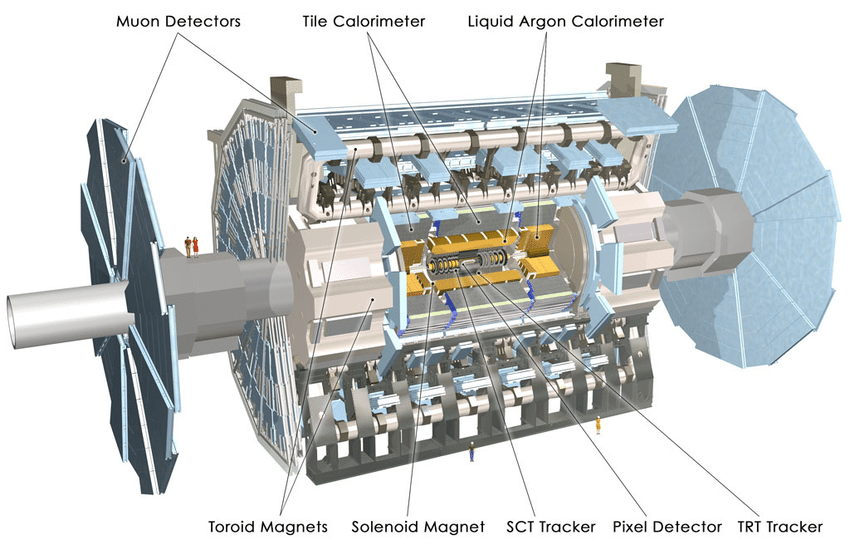
\includegraphics[width=0.5\textwidth]{figures/theoryFigs/atlasDetector.png}
\caption{Schematic of the ATLAS detector~\cite{Collaboration_2008}}
\end{figure}


The detector is cylindrically shaped which covers close to 4$\pi$ in solid angle. It has a length of 44 m, a diameter of 25 m and a mass of 7000 tons. ATLAS consists of four main sub-detectors arranged in concentric cylindrical layers around the beam pipe. These include the inner detector, the electromagnetic calorimeter, the hadronic calorimeters and the muon spectrometer. The sub-detectors record the momenta, energies and trajectories of different particles produced in the collider, allowing for the reconstruction and identification of these particles to be used in physics analyses.

\subsection{Coordinate System and Kinematics}

The ATLAS detector adopts a right-handed coordinate system. The origin is at the nominal interaction point and the beam direction defines the $z$-axis. The $x-y$ plane (or transverse plane) is perpendicular to the beam line, with the $x$-axis pointing towards the centre of the LHC ring and the $y$-axis pointing upwards towards the Earth's surface. An azimuthal angle, $\phi$, with $\phi \in \[ -\frac{\pi}{2}, \frac{\pi}{2} \] $ is defined in 



Physical dimensions, properties (mass). Coordinate system. Definition of $\Delta R$, $\eta$.\\\\
In the next subsections:\\
Where are different particles detected? How are they detected at each part of the detector? How well do the different parts detect the different particles and how do they take advantage of different particle properties each part wishes to detect in an engineering/physics perspective (e.g. why we WANT some particles to get detected at some parts of the detector and how we do this (by use of correct materials which interact specifically with those particles which we wish to measure and NOT with other particles))

\subsection{Tracking Detectors}
\subsection{Calorimeter System}
\subsubsection{Electromagnetic Calorimeter}
\subsubsection{Hadronic Calorimeter}
\subsection{Muon Spectrometer}
\subsection{Trigger and Data Acquisition System}
\subsection{Particle Identification} 
